\subsection{BRI1 Receptor Component}

From the description of the BL concentration function in Equation \eqref{bl} we can derive a formula for the concentration of bound BRI1 receptors at any position in the root. To do this, we use the equilibrium and mass-balance equations for the BRI1 receptor network introduced by \cite{vanesse2012}.

\begin{equation}
    \label{eq}
    [\text{BRI1 BL}] = \frac{[\text{BRI1}_{\text{free}}] \cdot [\text{BL}_{\text{free}}]}{K_{d}}
\end{equation}

\begin{equation}
    \label{mb}
\begin{aligned}
    \relax
    [\text{BRI1}] &= [\text{BRI1 BL}] + [\text{BRI1}_{\text{free}}]\\[5pt]
    [\text{BL}] &= [\text{BRI1 BL}] + [\text{BL}_{\text{free}}]
\end{aligned}
\end{equation}

In the equations above, $[\text{BRI1 BL}]$ denotes the concentration of bound BRI1 receptors, which are assumed to bind at a ratio of one molecule to one monomer (\cite{vanesse2012}). $K_{d}$ is the BL dissociation constant. Additionally, $[\text{BRI1}_{\text{free}}]$ and $[\text{BL}_{\text{free}}]$ denote the unbound BRI1 and BL concentrations respectively, while $[\text{BL}]$ and $[\text{BRI1}]$ represent the total BRI1 and BL concentrations. To further simplify our model, we can express $[\text{BRI1 BL}]$ as a function of $[\text{BRI1}]$ and $[\text{BL}]$ by substituting \eqref{mb} into \eqref{eq} to get:


\begin{equation}
\label{bri1-1}
[\text{BRI1 BL}] = \frac{([\text{BRI1}] - [\text{BRI1 BL}])([\text{BL}] - [\text{BRI1 BL}])}{K_{d}}
\end{equation}

\begin{equation}
\label{bri1-2}
K_{d} \cdot [\text{BRI1 BL}] = [\text{BRI1}] \cdot [\text{BL}] - ([\text{BL}] + [\text{BRI1}]) \cdot [\text{BRI1 BL}] + [\text{BRI1 BL}]^{2}
\end{equation}

\begin{equation}
\label{bri1-3}
[\text{BRI1 BL}]^{2} - ([\text{BL}] + [\text{BRI1}] + K_{d}) \cdot [\text{BRI1 BL}] + ([\text{BRI1}] \cdot [\text{BL}]) = 0
\end{equation}

Now, we can use the quadratic formula to determine the positive value of $[\text{BRI1 BL}]$ for which \eqref{bri1-3} holds. This gives us a formula for $[\text{BRI1 BL}]$ in terms of $[\text{BRI1}]$ and $[\text{BR}]$, where $A = ([\text{BL}] + [\text{BRI1}] + K_{d})$.

\begin{equation}
\label{bri1}
[\text{BRI1 BL}] = \frac{A - \sqrt{A^{2} - 4 \cdot [\text{BRI1}] \cdot [\text{BL}]}}{2}
\end{equation}

Empirical research gives us estimates for the values of $[\text{BRI1}]$ and $K_{d}$. \cite{vanesse2012} estimate the BRI1 receptor concentration to be $62 \pm 4 \nm$ in wild type roots. Values for the BL dissociation constant $K_{d}$ range from $7.4 \nm$ to $15 \nm$ (\cite{wang2001}) up to $55 \nm$ (\cite{cano-delgado2004}). For the models presented in the forthcoming sections, we will take $[\text{BRI1}] = 62 \nm$  and $K_{d} = 10\nm$. Using these parameters along with the formula in equation \eqref{bri1} we get the $[\text{BRI1 BL}]$ function shown in Figure \ref{fig:bri1-function}.

\begin{figure}
    \centering
    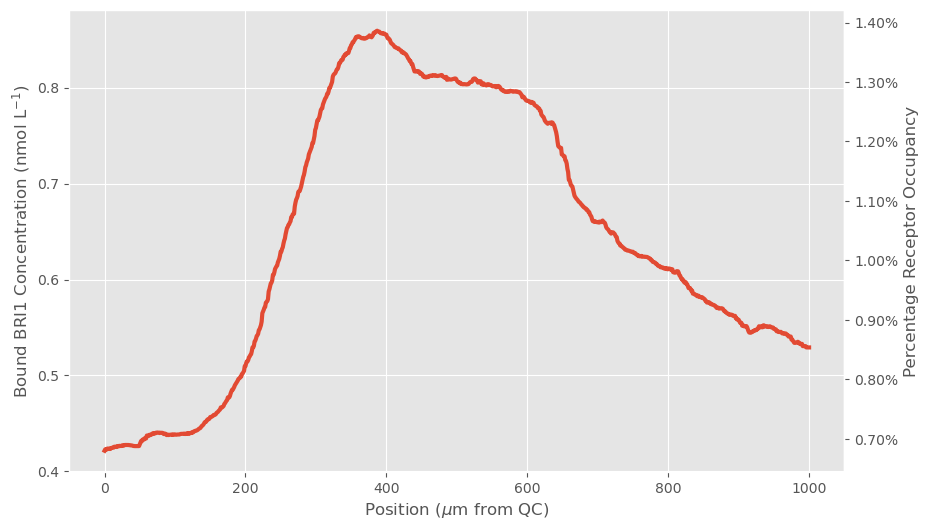
\includegraphics[width=13cm]{img/bri1-function.png}
    \caption{Plot of bound receptor concentration (left axis) measured in $\nm$ as well as receptor occupancy percentage (right axis). Due to the fact that $[\text{BL}] \ll [\text{BRI1}]$ the $[\text{BRI1 BL}]$ function is approximately equal to the $[\text{BL}]$ function up to some scalar multiple. }
    \label{fig:bri1-function}
\end{figure}


\medskip

Our model makes the assumption that all BRI1 receptors are localized to the cell membrane. Additionally, it assumes that the law of mass action is a reasonable approximation for the diffusing BL ligand binding to the static BRI1 receptors. We believe this decision is justified due to the low percentage occupancy of the BRI1 receptors, which suggests that any free BL ligand will have many oppourtunities to bind to a receptor. Further modelling of the BRI1 receptor network using the physical properties of the system would help to clarify and refine these assumptions.


